\documentclass{standalone}

\usepackage{tikz}
\usetikzlibrary{shapes}
\begin{document}


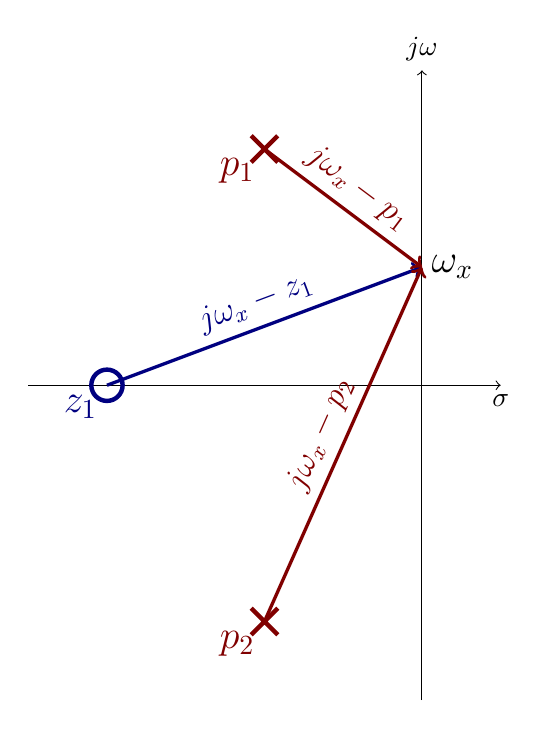
\begin{tikzpicture}
  \draw[->] (-5,0) -- (1,0) node[below] {$\sigma$};
  \draw[->] (0,-4) -- (0,4) node[above] {$j\omega$};

  \node[right, font = \Large, color = black] at (0, 1.5) {$\omega_x$};
  \node[circle, ultra thick, color = blue!50!black, draw, inner sep=4pt] at (-4,0) {};
  \node[below left, font = \Large, color = blue!50!black] at (-4, 0) {$z_1$};

  \draw[->,very thick, color=blue!50!black] (-4,0) -- node[midway, sloped, above, font =\large] {$j\omega_x - z_1$} (0,1.5);

  \node[cross out, ultra thick, color = red!50!black, draw, inner sep=4pt] at (-2,3) {};
  \node[cross out, ultra thick, color = red!50!black, draw, inner sep=4pt] at (-2,-3) {};
  \node[below left, color = red!50!black, font = \Large] at (-2, 3) {$p_1$};
  \node[below left, color = red!50!black, font = \Large] at (-2, -3) {$p_2$};

  \draw[->,very thick, color=red!50!black] (-2,3) -- node[midway, sloped, above, font =\large] {$j\omega_x - p_1$} (0,1.5);
  \draw[->,very thick, color=red!50!black] (-2,-3) -- node[midway, sloped, above, font =\large] {$j\omega_x - p_2$} (0,1.5);


\end{tikzpicture}

\end{document}
